\documentclass[10pt]{article}

\usepackage[margin=0.9in,headheight=14pt]{geometry}
\usepackage[T1]{fontenc}
\usepackage[utf8]{inputenc}
\usepackage{booktabs}
\usepackage{longtable}
\usepackage{tabularx}
\usepackage{array}
\usepackage{url}
\usepackage{hyperref}
\usepackage{graphicx}
\usepackage{amsmath}
\usepackage[table]{xcolor}
\usepackage{caption}
\usepackage{pdflscape}
\usepackage{fancyhdr}

\hypersetup{
  colorlinks=true,
  linkcolor=black,
  citecolor=black,
  urlcolor=blue
}
\renewcommand{\thefigure}{S\arabic{figure}}
\renewcommand{\thetable}{S\arabic{table}}
\renewcommand{\figurename}{Supplementary Figure}
\renewcommand{\tablename}{Supplementary Table}
\emergencystretch=2em
\captionsetup{font=small,labelfont=bf,justification=raggedright,singlelinecheck=false,skip=6pt,hypcap=false}
\definecolor{suppblue}{HTML}{286A8E}
\definecolor{suppbluepale}{HTML}{EAF2F6}
\definecolor{supprow}{HTML}{F6F4EF}
\definecolor{supprule}{HTML}{B8C7CE}
\arrayrulecolor{supprule}
\setlength{\LTcapwidth}{0.92\textwidth}
\setlength{\parindent}{0pt}
\setlength{\parskip}{5pt}
\pagestyle{fancy}
\fancyhf{}
\lhead{\small Trimole-Hybrid ADMET}
\rhead{\small Supplementary Information}
\cfoot{\small S\thepage}
\renewcommand{\headrulewidth}{0.3pt}
\renewcommand{\footrulewidth}{0pt}

\newcolumntype{Y}{>{\raggedright\arraybackslash}X}
\newcommand{\suppnote}[1]{\section*{#1}\addcontentsline{toc}{section}{#1}}
\newcommand{\suppnoteplain}[1]{\section*{#1}\addcontentsline{toc}{section}{#1}}
\newcommand{\suppsubnote}[1]{\subsection*{#1}\addcontentsline{toc}{subsection}{#1}}
\newcommand{\used}{\textcolor{suppblue}{\textbullet}}
\newcommand{\scorepm}[2]{\begin{tabular}{@{}c@{}}$#1$\\[-1pt]$\pm\;#2$\end{tabular}}

\title{Supplementary Information for\\Task-wise multimodal model selection and ensemble learning for molecular ADMET prediction}
\author{Zhensheng Luo, Dachen Huang, Yanruisheng Shao, Qinze Yu and Yu Li}
\date{}

\begin{document}
\begin{titlepage}
\thispagestyle{empty}
\raggedright
\vspace*{1.0cm}
{\Large\bfseries Supplementary Information\par}
\vspace{0.8cm}
{\LARGE\bfseries\begin{minipage}{0.88\textwidth}
\raggedright Task-wise multimodal model selection and ensemble learning for molecular ADMET prediction
\end{minipage}\par}
\vspace{0.7cm}
{\large Zhensheng Luo, Dachen Huang, Yanruisheng Shao, Qinze Yu and Yu Li\par}
\vspace{1.0cm}
\noindent\rule{\textwidth}{0.6pt}
\vspace{0.35cm}

\begin{minipage}{0.92\textwidth}
This file contains Supplementary Notes 1--8, Supplementary Figures S1--S2 and Supplementary Tables A--C, S1--S24 and S4e for the Trimole-Hybrid ADMET study.
\end{minipage}

\vfill
Repository: \url{https://github.com/dchen0212/trimole_hybrid}
\end{titlepage}
\setcounter{page}{1}
\tableofcontents
\clearpage

\suppnoteplain{Supplementary Overview}

This Supplementary Information provides the benchmark protocol, reference snapshot, task-configuration records, ablation settings, case-study checks, metric interpretation, software environment and revision audits for the Trimole-Hybrid ADMET study. It does not add leaderboard claims beyond the main text. Complete machine-readable tables are provided in the GitHub repository under \href{https://github.com/dchen0212/trimole_hybrid/tree/main/supplementary_tables}{\texttt{supplementary\_tables/}}, including the consolidated supplementary workbook and the individual CSV files.

Supplementary Tables A--C are compact tables included in this PDF for readability. Supplementary Tables S1--S24 and S4e are the machine-readable workbook and CSV tables used as the complete record for the benchmark, ablations, case-study checks, provenance, leakage audit, controlled baselines, uncertainty and selection stability.

\textbf{Supplementary file guide.}
Supplementary Tables A--C and Supplementary Figures S1--S2 provide compact PDF summaries. Supplementary Tables S1--S24 and S4e provide the complete machine-readable record. Table S1 reports the corrected 22-task benchmark; Tables S2, S13 and S15 record task configurations and selection evidence; Tables S3 and S14 record the fixed public-reference snapshot; Tables S4, S4e and S23 record scale-aware ablations and selection stability; Tables S7--S10 and S17 record molecule-level case-study checks; Tables S11 and S19 record split, source, endpoint and applicability provenance; Table S20 records cross-task overlap and leakage-safe correction; Table S21 records controlled baselines and matched-budget AutoML; Table S22 records uncertainty and subgroup analysis; Table S24 records an expanded nine-family stable common-pool sensitivity analysis and the preceding 15-family eligibility audit; Table S16 records metric interpretation; and Table S18 records the software environment.

\suppnote{Supplementary Note 1: Benchmark Protocol and Frozen Reference Snapshot}

All benchmark results used the 22 tasks in the TDC ADMET benchmark group and the official scaffold splits. For each task, the official training and validation sets were used for model fitting, model choice and calibration. The official test set was evaluated only after the task-specific model configuration had been fixed.

The public TDC leaderboard is not a set of baselines rerun by us under one budget. We therefore used a fixed leaderboard snapshot recorded on 15 May 2026. The top-1 reference score, task rank and metric direction were copied from that snapshot and treated as external comparison metadata. These values were not used to choose model families, blend weights, seed sets, ablation variants or molecule-level examples.

A positive direction-normalized margin means that Trimole-Hybrid matched or exceeded the fixed public top-1 score after accounting for metric direction. This comparison should not be read as a head-to-head rerun of every public baseline.

Supplementary Table S14 records the snapshot date, the public reference method name when available, the reference score, the Trimole-Hybrid score, the direction-normalized margin and the rank metadata.

\suppnote{Supplementary Note 2: Candidate Pool and Task Configuration Records}

For each task, Trimole-Hybrid selected one model configuration from a fixed candidate pool. The pool included sequence-based encoders, graph-based encoders, EPT/3D predictors, chemistry-prior models, seed-bagged variants and prediction-level ensembles. Selection used only the official training/validation split or scaffold cross-validation within the training/validation partition.

The selected-configuration ledger records the model family, task configuration, seed usage, ensemble rule, EPT/3D use and source files. Supplementary Table A provides a compact version of that ledger. Full candidate identifiers, weights, seed definitions, source files and ablation configurations are given in Supplementary Tables S2--S2d. Supplementary Tables S13 and S15 give the number of checked variants and the candidate-pool scope for each task.

\suppnote{Supplementary Note 3: Model Formulation and Task Configuration Matrix}

The main Methods section is short to meet the Bioinformatics length constraint. Here we give the notation used for implementation. For task $t$, let $D_t^{\mathrm{train}}$, $D_t^{\mathrm{val}}$ and $D_t^{\mathrm{test}}$ denote the official training, validation and test splits. Candidate parameters were fitted on $D_t^{\mathrm{train}}$ (or on inner scaffold folds formed without $D_t^{\mathrm{test}}$), and candidate configurations were ranked on $D_t^{\mathrm{val}}$. Only after a configuration had been frozen was it refitted, where applicable, on
\begin{equation}
  D_t^{\mathrm{refit}} = D_t^{\mathrm{train}} \cup D_t^{\mathrm{val}}.
\end{equation}
The refit did not reuse $D_t^{\mathrm{val}}$ as an early-stopping set. The official test set was then evaluated once for the frozen configuration. Thus, $D_t^{\mathrm{val}}$ was not simultaneously part of candidate fitting and candidate ranking, and $D_t^{\mathrm{test}}$ was not used for model-family choice, blend-weight choice or seed choice.

For family-transfer candidates, molecular identities were compared across tasks using the connectivity block of an RDKit-generated InChIKey. During candidate selection for target task $t$, pooled source-training rows matching any molecule in $D_t^{\mathrm{val}}$ or $D_t^{\mathrm{test}}$ were removed. During final refitting, pooled source training/validation rows matching any molecule in $D_t^{\mathrm{test}}$ were removed. The overlap audit reports pre-filter and post-filter row counts without publishing test-molecule identities.

For molecule $x_i$, the candidate models used the following molecular representations:
\begin{equation}
  \mathcal{V}(x_i)=
  \{v_{\mathrm{seq}}(x_i), v_{\mathrm{graph}}(x_i), v_{\mathrm{3D}}(x_i), v_{\mathrm{chem}}(x_i)\},
\end{equation}
where the four terms denote sequence, molecular graph, geometry-sensitive and chemistry-prior representations, respectively. Each available representation is mapped to an embedding or feature vector,
\begin{equation}
  h_i^{(m)} = f_m\!\left(v_m(x_i)\right), \qquad m \in \mathcal{M}_t,
\end{equation}
where $\mathcal{M}_t$ is the modality set available for task $t$. Sequence candidates used canonical SMILES language-model representations. Graph candidates used pretrained molecular graph embeddings. EPT/3D candidates used geometry-sensitive or task-tailored structural information. Chemistry-prior candidates used fingerprints, descriptors and tabular chemical features.

For neural fusion candidates, modality-specific embeddings were projected into a shared hidden space,
\begin{equation}
  z_i^{(m)} = \phi_m\!\left(h_i^{(m)}\right).
\end{equation}
In gated fusion variants, projected embeddings were combined as
\begin{equation}
  h_i^{\mathrm{fuse}} =
  \sum_{m \in \mathcal{M}_t}\alpha_{i,t}^{(m)} z_i^{(m)},
  \qquad
  \sum_{m \in \mathcal{M}_t}\alpha_{i,t}^{(m)}=1,
\end{equation}
where $\alpha_{i,t}^{(m)}$ denotes a sample- or task-dependent modality weight. MLP-fusion variants concatenated projected embeddings instead of applying gates. The task-specific head then produced
\begin{equation}
  \hat{y}_{i,t}=g_t\!\left(h_i^{\mathrm{fuse}}\right),
\end{equation}
with $g_t$ defined as a classification or regression head according to the official TDC task type.

Some candidates combined predictions from fixed base models rather than changing the molecular encoders. For task $t$, an ensemble candidate can be written as
\begin{equation}
  \hat{y}_{i,t}^{\mathrm{ens}}
  =
  \sum_{k=1}^{K_t} w_{k,t}\,T_t\!\left(\hat{y}_{i,t}^{(k)}\right),
  \qquad
  \sum_{k=1}^{K_t} w_{k,t}=1,
\end{equation}
where $\hat{y}_{i,t}^{(k)}$ is the prediction from candidate $k$, $w_{k,t}$ is a validation-selected or predefined ensemble weight, and $T_t(\cdot)$ is a task-dependent transformation such as identity, logit, rank or z-score transformation. Identity transformations were used for raw regression-value blending. Rank- or z-score-based transformations were used for Spearman-style tasks.

Task-specific selection used validation data only. Let $\mathcal{C}_t$ denote the candidate set for task $t$. The selected configuration was
\begin{equation}
  c_t^{\ast}
  =
  \arg\max_{c \in \mathcal{C}_t}
  S_t^{\mathrm{val}}\!\left(c;D_t^{\mathrm{val}}\right),
\end{equation}
where $S_t^{\mathrm{val}}$ is the official task metric after applying the appropriate metric direction. After selection and optional refitting, $c_t^{\ast}$ was fixed and evaluated on the official test split to obtain the final reported score,
\begin{equation}
  S_t^{\mathrm{test}}
  =
  S_t\!\left(c_t^{\ast};D_t^{\mathrm{test}}\right).
\end{equation}
The same validation-only rule was used for the final model and for the component-removal ablations.

{\footnotesize
\renewcommand{\arraystretch}{1.08}
\setlength{\tabcolsep}{3.4pt}
\rowcolors{2}{supprow}{white}
\begin{longtable}{p{2.45cm} p{1.55cm} p{4.15cm} c c c c c c}
\caption*{\textbf{Supplementary Table A.} Compact component matrix for the fixed 22-task model configurations. A filled entry indicates that the component was used in the final configuration for that task. Full configuration records are provided in Supplementary Tables S2--S2d.}\\
\toprule
\rowcolor{suppbluepale}
Dataset & Metric & Fixed model family & Chem & Seq & Graph & EPT/3D & Blend & Bag \\
\midrule
\endfirsthead
\toprule
\rowcolor{suppbluepale}
Dataset & Metric & Fixed model family & Chem & Seq & Graph & EPT/3D & Blend & Bag \\
\midrule
\endhead
TDC.Bioav & AUROC & Fixed chem ExtraTrees & \used &  & \used &  &  & \used \\
TDC.Caco2 & MAE & Fixed chem ExtraTrees & \used & \used & \used &  &  & \used \\
TDC.HIA & AUROC & Task-specific chem blend & \used &  &  &  & \used & \used \\
TDC.Lipo & MAE & XL/chem hybrid blend & \used & \used & \used & \used & \used & \used \\
TDC.Pgp & AUROC & KPGT/EPT logit blend &  & \used & \used & \used & \used &  \\
TDC.AqSol & MAE & FP-XGB/KPGT-EPT/XL blend & \used & \used & \used & \used & \used &  \\
TDC.BBB & AUROC & Descriptor ExtraTrees & \used &  &  &  &  &  \\
TDC.PPBR & MAE & KPGT/fingerprint blend & \used &  & \used &  & \used & \used \\
TDC.VD & Spearman & KPGT/EPT rank blend & \used &  & \used & \used & \used & \used \\
TDC.CYP2C9-S & AUPRC & Fixed chem XGBoost & \used & \used & \used & \used &  & \used \\
TDC.CYP2C9-I & AUPRC & Fixed chem XGBoost & \used &  & \used & \used &  & \used \\
TDC.CYP2D6-S & AUPRC & AP/XL/descriptor blend & \used & \used &  & \used & \used & \used \\
TDC.CYP2D6-I & AUPRC & KPGT/EPT/FP rank blend & \used &  & \used & \used & \used & \used \\
TDC.CYP3A4-S & AUROC & Family-transfer FP-XGBoost & \used &  &  &  &  &  \\
TDC.CYP3A4-I & AUPRC & XL/KPGT-EPT logit blend & \used & \used & \used & \used & \used & \used \\
TDC.CL-Hepa & Spearman & Family-transfer FP-XGBoost & \used &  &  &  &  &  \\
TDC.CL-Micro & Spearman & KPGT/EPT seedbag &  &  & \used & \used & \used & \used \\
TDC.Half\_Life & Spearman & C+K descriptor/z-score blend & \used & \used & \used &  & \used & \used \\
TDC.AMES & AUROC & Repeated fingerprint XGBoost & \used &  &  &  &  & \used \\
TDC.DILI & AUROC & XL/KPGT-EPT raw blend & \used & \used & \used & \used & \used & \used \\
TDC.hERG & AUROC & Fixed chem ExtraTrees & \used & \used &  & \used &  & \used \\
TDC.LD50 & MAE & Fixed chem XGBoost & \used & \used & \used & \used &  & \used \\
\bottomrule
\end{longtable}
\rowcolors{2}{}{}
}

The source-provenance check found that the v36 main results used official TDC benchmark splits and did not use \texttt{data\_new}. Supplementary Table S11 gives the main-result source check. The ablation README records the same rule: fixed candidate families were rerun on official-split embeddings or fingerprints, validation data were used for selection, and test scores were used only after selection.

Supplementary Table S13 is a one-row-per-task manifest. It links the final score, selected candidate, model-family summary, seed definition, checked-variant count, candidate-pool scope, selection summary, test-score source file, official-split provenance and component flags. Supplementary Table S15 summarizes the validation-only selection record for each task and points to the selected configuration and the five component-removal comparators.

\suppnote{Supplementary Note 4: Formal Ablation Protocol}

The ablations quantified the contribution of each major component to the final benchmark scores. The variants were: full Trimole-Hybrid, no task-adaptive selection, no chemistry sidecar, no EPT/3D, no prediction-level ensemble and a single-seed version of seed-bagged tasks where available.

For each component-removal ablation, task-wise selection was repeated with the same validation-only rule after removing that component class. The single-seed variant reports the closest available canonical single-seed candidate. These variants were not submitted as independent leaderboard entries, so they should be read as within-study comparisons against the full model. The ablation source files also record that the reruns used official-split embeddings, fingerprints and fixed heads, and that \texttt{data\_new} was not used.

\begin{center}
\makebox[\textwidth][c]{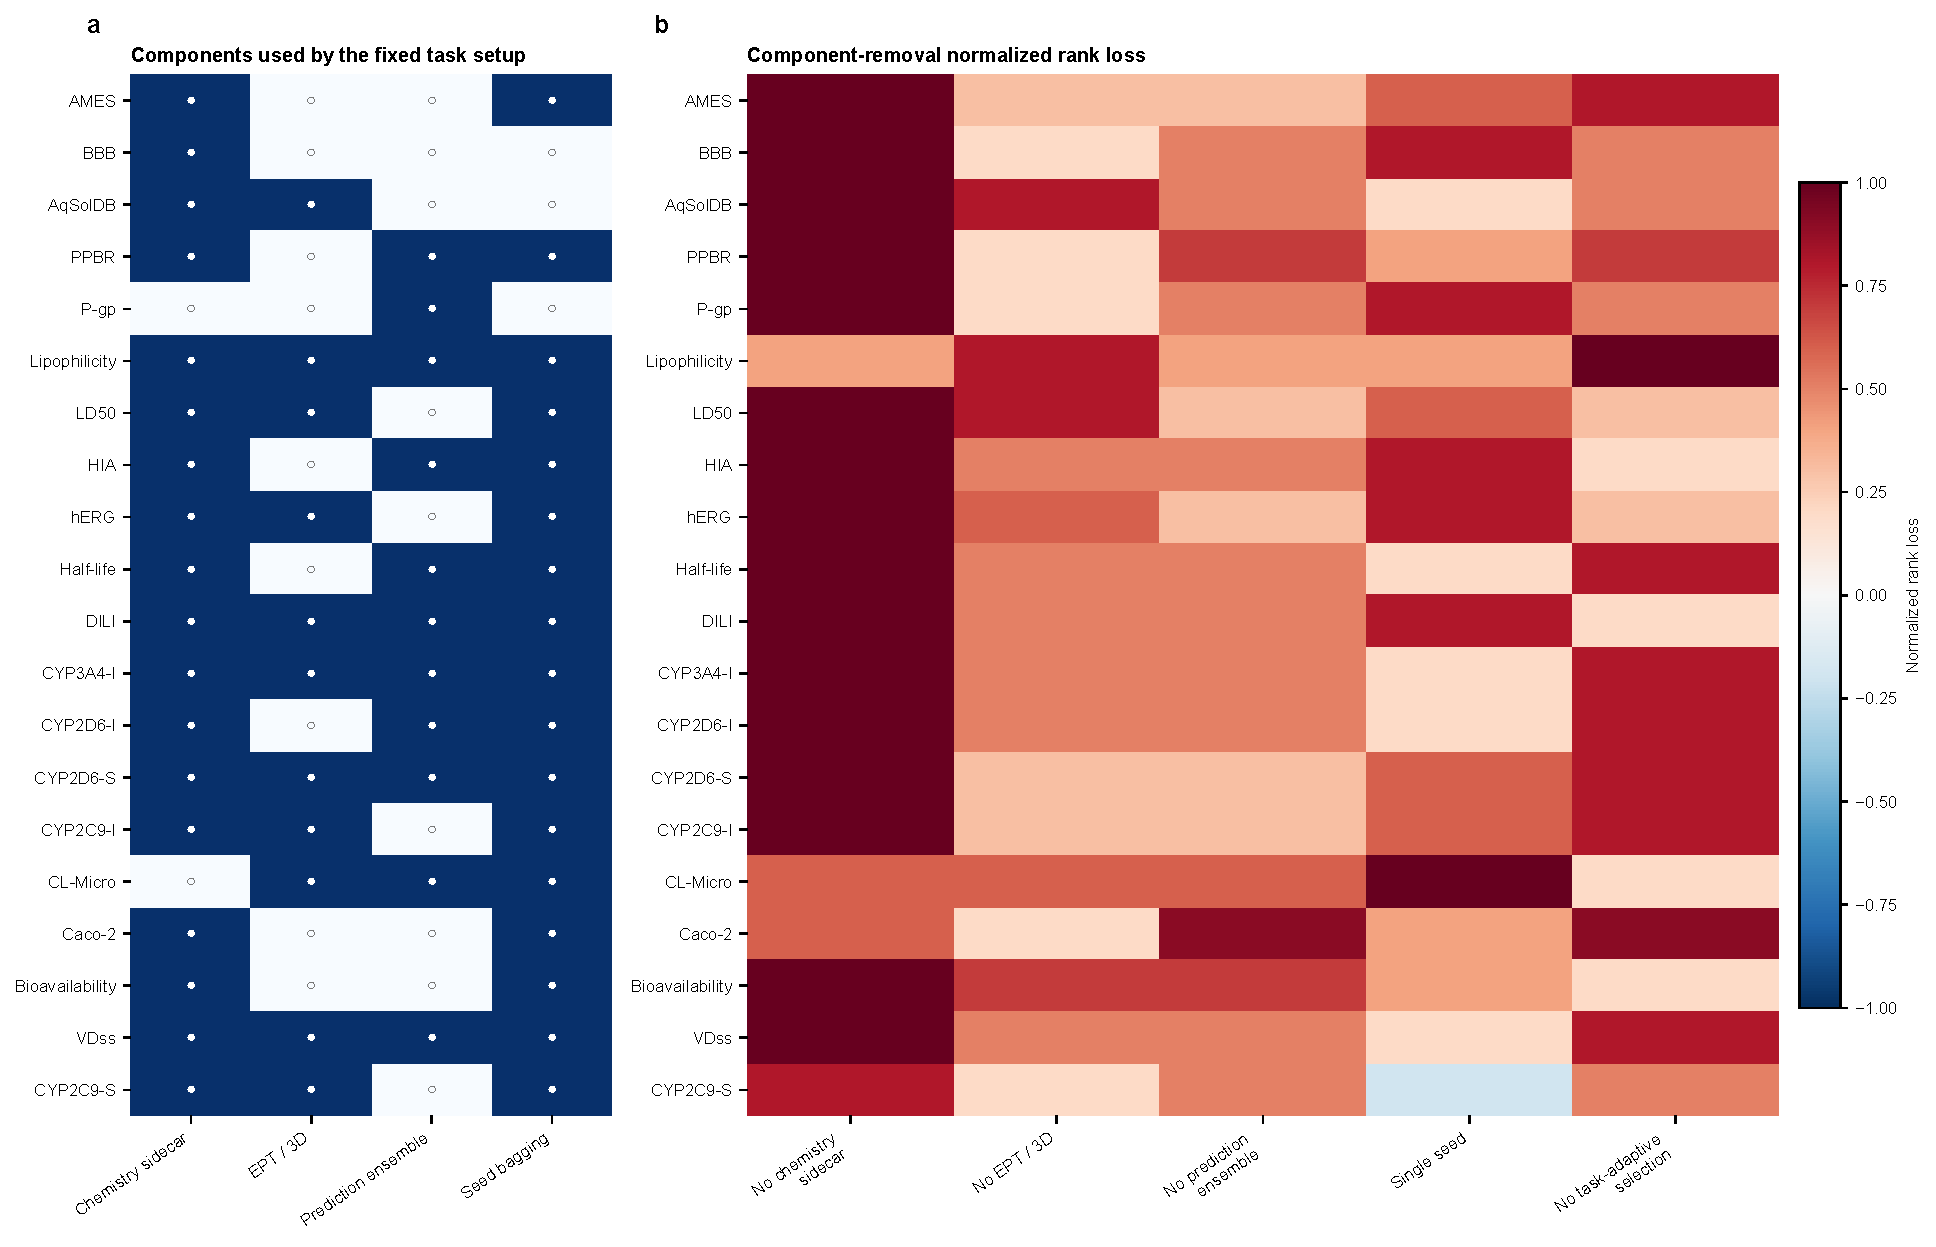
\includegraphics[width=1.04\textwidth]{supplementary_figures/Supplementary_Figure_S1_component_ablation_combined.pdf}}
\vspace{6pt}
\begin{minipage}{\textwidth}
\captionof{figure}{Task-wise component usage and scale-free component-removal effects. \textbf{a}, Component map for the 22 fixed TDC ADMET task configurations. Filled circles indicate components used in the final configuration; open circles indicate components not used. \textbf{b}, Within-task normalized rank loss after removing each component class. Positive values indicate a worse within-task rank than the corrected full configuration, zero indicates a tie and negative values indicate an improved rank after restriction. Exact task-level scores, ranks and stability statistics are provided in Supplementary Table S23. Task labels use abbreviated dataset codes; full endpoint names are listed in Supplementary Table S1. \textbf{Alt text:} A two-panel matrix and heatmap show which chemistry, geometry, ensemble and seed-bagging components each of 22 tasks uses and the scale-free normalized rank loss after each component restriction.}
\label{fig:supp_component_ablation}
\end{minipage}
\end{center}

\begin{figure}[htbp]
\centering
\setlength{\fboxsep}{7pt}
\begin{minipage}{0.96\textwidth}
\centering
\fbox{\parbox{0.82\textwidth}{\centering \textbf{1. Frozen task split and feature extraction}\\Encoder fitting or fixed feature extraction uses no official test labels.}}

$\Downarrow$

\fbox{\parbox{0.82\textwidth}{\centering \textbf{2. Base-model fitting}\\Candidate parameters are fitted on training data or inner training folds.}}

$\Downarrow$

\fbox{\parbox{0.82\textwidth}{\centering \textbf{3. Validation-only decisions}\\Hyperparameters, candidate identity, blend weights, calibration and candidate ranking are fixed using validation data. A machine-readable selection manifest is written here.}}

$\Downarrow$

\fbox{\parbox{0.82\textwidth}{\centering \textbf{4. Frozen refit}\\The selected configuration is refitted on training plus validation data without changing its identity or settings.}}

$\Downarrow$

\fbox{\parbox{0.82\textwidth}{\centering \textbf{5. Test reporting only}\\Official test labels are first read by the scoring phase after predictions and their manifest have been written.}}
\end{minipage}
\caption{Leakage-controlled development and evaluation protocol. The test split can be featurized without labels for final prediction, but its labels are inaccessible to selection and refitting code. Family-transfer candidates additionally remove source molecules matching target validation or test identities during selection and target test identities during final refitting. \textbf{Alt text:} Five vertically ordered boxes separate frozen splitting and feature extraction, base-model fitting, validation-only decisions, frozen train-plus-validation refitting and final test-only scoring.}
\label{fig:supp_protocol}
\end{figure}

\clearpage

\suppnote{Supplementary Note 5: Molecule-Level Case-Study Audit}

The main text contains two molecule-level sensitivity examples. Both were chosen after the task models had been fixed. They were not used for model selection, task promotion, ablation design or leaderboard comparison. They report score changes for individual molecules and matched local replacements. They do not prove causal pharmacophores.

The two examples have different replay and label status. The AMES example has an official-test label and a saved full prediction for the original molecule, but its perturbation sweep used a reconstructed task model. We therefore label it as reconstruction-based sensitivity, not exact full-ensemble attribution. The Deutivacaftor example uses the replayed TDC P-gp-inhibition pipeline for both the external molecule and its matched local replacement, but has no matched experimental inhibition label. It therefore has stronger replay status but weaker outcome evidence. Both examples remain model-sensitivity checks, not mechanistic or prospective-accuracy claims.

\begin{table}[htbp]
\centering
\caption*{\textbf{Supplementary Table B.} Two molecule-level sensitivity examples shown in Figure 4. Full details are provided in Supplementary Table S7.}
\small
\renewcommand{\arraystretch}{1.12}
\begin{tabularx}{\textwidth}{p{2.5cm} p{2.0cm} p{1.2cm} p{1.8cm} p{1.8cm} Y}
\toprule
\rowcolor{suppbluepale}
Case & Task & Label status & MiniMol output & Trimole output & Sensitivity status \\
\midrule
AMES test\_297 & AMES & 1 & 0.293194 & 0.894085 & Original molecule uses a saved Trimole-Hybrid prediction; perturbation uses a reconstructed AMES model and is not exact full-ensemble attribution. \\
Deutivacaftor & P-gp inhibition & None & \scorepm{0.746979}{0.064799} & \scorepm{0.914545}{0.021395} & Exact replayed endpoint pipeline; O-to-CH2 matched replacement reduced the model output to \scorepm{0.729853}{0.149185}; no correctness claim is made. \\
\bottomrule
\end{tabularx}
\end{table}

External molecule candidates were converted to canonical SMILES and compared with the corresponding official TDC task splits. Candidates found in the training set were excluded from main-text use. For Deutivacaftor, no canonical SMILES overlap was found in the Pgp\_Broccatelli training, validation or test split. Because that benchmark endpoint is P-gp inhibition and no matched experimental inhibition label was identified for Deutivacaftor, this example is treated only as an unlabeled output-sensitivity check, not as a new benchmark task or a labeled external validation.

Several molecule-level candidates were examined but not used in the main sensitivity figure. A candidate was not promoted when an exact replay path was not available under the archived inference setting, the matched replacement did not yield a stable sensitivity pattern, or the available evidence could not support even a constrained sensitivity interpretation. Supplementary Table S17 lists the promoted and non-promoted molecule-level examples. A case was eligible for main-text use only if it had an explicit label-status field, no prohibited training-set overlap for external cases, a reportable model output and a replay-status label. An unlabeled external molecule can support sensitivity analysis but not correctness or external-validation claims.

\begin{table}[htbp]
\centering
\caption*{\textbf{Supplementary Table C.} Selected case-study candidates that were not used in the main figure. Full details are provided in Supplementary Table S10.}
\small
\renewcommand{\arraystretch}{1.12}
\begin{tabularx}{\textwidth}{p{2.6cm} p{1.8cm} Y Y}
\toprule
\rowcolor{suppbluepale}
Candidate & Task & Main issue & Final use \\
\midrule
BBB external candidates & BBB & The archived replay path did not meet the criteria for main-text interpretation, and no MiniMol-wrong/Trimole-correct external candidate was found. & Not used in the main figure. \\
Ritlecitinib & CYP3A4-S & Original prediction comparison was promising, but matched replacement did not give a stable sensitivity signal. & Not used in the main figure. \\
Mavorixafor & P-gp & Boundary case with weak replacement evidence. & Not promoted. \\
AqSol external candidates & AqSol & Exact arbitrary-SMILES external inference was not available in the archived replay setting. & Not promoted. \\
PPBR external candidates & PPBR & External predictions remained near-reconstruction or proxy rather than exact replay. & Not promoted. \\
\bottomrule
\end{tabularx}
\end{table}

For this reason, AMES is labeled as an official-label example with reconstruction-based perturbation sensitivity, whereas Deutivacaftor is labeled as an unlabeled external example with exact endpoint replay. The two evidence types should not be treated as equivalent.

\suppnote{Supplementary Note 6: Metric Direction and Endpoint Scale}

The benchmark uses classification metrics, absolute-error regression metrics and rank-correlation metrics. Direction-normalized margins were used only to compare these task-level scores in one table. For AUROC, AUPRC and Spearman correlation, the margin is the Trimole-Hybrid score minus the fixed reference score. For MAE, the margin is the reference MAE minus the Trimole-Hybrid MAE. Positive margins therefore indicate matched or better performance relative to the fixed reference.

Supplementary Table S16 records the metric direction, margin formula and label-scale notes used in the manuscript. AUROC, AUPRC and Spearman correlation are task-level metrics. A single molecule can have a predicted classification score, and a single MAE-task molecule can have an absolute error on the reported label scale. A single molecule cannot have its own AUROC, AUPRC or Spearman value. Spearman-task molecule examples should therefore be read as continuous-score examples, not as single-molecule rank-correlation errors.

\suppnote{Supplementary Note 7: Software Environment and Data Availability}

Supplementary Table S18 reports the software environments used for model assembly, official-split tabular models and graph-feature extraction. The public project repository is available at \url{https://github.com/dchen0212/trimole_hybrid}. The principal benchmark environment used Python 3.10.20 with RDKit 2026.03.1, scikit-learn 1.7.2, XGBoost 3.2.0 and PyTorch 2.5.1 with CUDA 12.1. KPGT feature extraction used a separate Python 3.10.19 environment with DGL 2.0.0 and PyTorch 2.1.2 with CUDA 12.1.

We include this environment table because some exploratory replay analyses depended on archived model files and package versions. AMES remains a valid benchmark result, but its perturbation result is labeled as reconstruction-based because the exact archived full-ensemble replay path was not available for arbitrary AMES SMILES.

All supplementary tables are included in the manuscript package under \texttt{supplementary\_tables/}. Source code, supplementary tables and lightweight audit manifests are available from the main manuscript repository. Large trained model binaries, cached embeddings and serialized estimators will be provided through archive or release assets where storage and licensing permit. The supplementary workbook remains the manuscript-level record for the benchmark, ablations and case-study checks.

\suppnote{Supplementary Note 8: Revision Audits, Controlled Comparisons and Statistical Analysis}

Supplementary Table S19 reports the named primary source, publication title, DOI or ChEMBL document accession, direct primary-source URL, separate TDC catalogue URL, endpoint definition, task type, label or unit, frozen train/validation/test counts, unique-SMILES count, class prevalence where applicable, observed label range, known measurement limitations and applicability-domain constraints for all 22 tasks. The 22 rows resolve to 15 distinct primary DOI/accession records because several tasks share a source publication or ChEMBL document. Counts refer to the exact frozen benchmark files used in this study. Row count and unique-molecule count are reported separately because repeated molecular strings occur in some datasets.

Supplementary Table S20 reports pairwise molecular overlap within the CYP-substrate and clearance families using the connectivity layer of an RDKit-generated parent InChIKey. It also records the source rows removed by the selection-stage and final-stage filters, the corrected test scores and the provenance files. The previously reported CYP3A4-substrate and hepatocyte-clearance family-transfer results were invalidated and replaced because their source pools contained target-test identities.

Supplementary Table S21 reports the consistently trained global single-model, per-task single-model, validation-selected top-2/top-3, uniform-average, out-of-fold stacking, matched-budget FLAML AutoML and Trimole-Hybrid comparisons. The controlled methods use the same frozen ChemBERTa, KPGT and EPT feature views, official splits and five fixed seeds. FLAML is limited to 60 seconds and 30 iterations per task and seed. All selection decisions use the official validation partition; the official test labels are inaccessible until the scoring phase. Trimole-Hybrid is the frozen submitted system and has a broader heterogeneous historical candidate pool, so this comparison does not claim identical candidate-pool coverage. Twenty-one tasks have five archived Trimole-Hybrid seed-level prediction arrays. BBB has one archived five-model ensemble prediction array plus historical five-run aggregate scores; its paired analysis uses the ensemble array. Because the controlled pool has exactly three views, top-3 and uniform averaging are identical by construction. Public leaderboard rows without sample-level predictions are retained only as descriptive external context.

Supplementary Table S22 reports 154 paired sample-level comparisons using 10,000 replicates, 95\% confidence intervals, two-sided bootstrap $p$ values and one Benjamini--Hochberg false-discovery-rate adjustment across all emitted task--comparator tests. Five-seed predictions are averaged per sample before metric recomputation. Trimole-Hybrid has the best point estimate on 21 of 22 controlled tasks and is significant against per-task single-view selection on 18 tasks after global correction. It also reports 132 task--descriptor--subgroup combinations with sample size, positive count and prevalence for classification tasks, matched scores and paired intervals. Of these, 131 pass the prespecified validity rule; the high-cLogP HIA subgroup is marked invalid because of insufficient class count and is not assigned an AUROC.

Supplementary Table S23 reports task-wise raw ablation metrics, normalized rank loss, validation-bootstrap candidate selection frequency, selection entropy and switching rate. The no-task-adaptive control is defined as one globally fixed candidate family selected by aggregate validation rank and applied unchanged to every task. Rank normalization is performed within each task and does not average raw AUROC, AUPRC, MAE and Spearman values.

Supplementary Table S24 extends the controlled analysis from three frozen feature views. Fifteen candidate families had complete validation and test prediction files for all 22 tasks and five fixed seeds, but validation-only diagnostics identified numerical divergence in all six unregularized deep linear heads. These six families were excluded globally, before test prediction contents were loaded; the eligibility decision and reason for every family are retained in Table S24f. The remaining nine stable XGBoost or Ridge families comprise 990 eligible candidate runs. Six rules---global single candidate, per-task single candidate, validation top-2 and top-3 averaging, uniform averaging and validation stacking---use exactly this common pool. Candidate identities and combination rules are frozen from validation predictions before test predictions are loaded. Test rows are then aligned by molecule, label and within-key occurrence against the current evaluation split. This identity-based audit excluded two legacy AqSolDB rows that were absent from the current 1,995-row test split; it did not truncate predictions by row position. The resulting 660 method--seed records and 132 method summaries contain finite, numerically plausible scores.

Against these six expanded-pool controls, Trimole-Hybrid ranked first by point estimate on 17 of 22 tasks and had mean within-task normalized rank utility 0.913. It had a positive paired point estimate in 19--21 tasks depending on the comparator. After one Benjamini--Hochberg correction across the 132 additional 10,000-replicate comparisons, 8--13 positive comparisons per comparator were significant. The negative result is retained: on hepatocyte clearance, uniform averaging, validation stacking and validation top-3 averaging significantly exceeded the leakage-corrected Trimole-Hybrid prediction. The expanded pool provides exact candidate-pool parity among the six control strategies, but it still does not reconstruct every heterogeneous historical candidate used to produce the frozen Trimole-Hybrid configurations; it is therefore a robustness analysis rather than proof of universal superiority.

\suppnote{Supplementary Tables}

{\footnotesize
\renewcommand{\arraystretch}{1.10}
\setlength{\tabcolsep}{4pt}
\rowcolors{2}{supprow}{white}
\begin{longtable}{p{1.1cm} p{5.0cm} p{8.0cm}}
\caption*{\textbf{Supplementary Table Inventory.} Complete machine-readable tables are provided in the supplementary workbook and as individual CSV files.}\\
\toprule
\rowcolor{suppbluepale}
Table & File & Description \\
\midrule
\endfirsthead
\toprule
\rowcolor{suppbluepale}
Table & File & Description \\
\midrule
\endhead
S1 & \path{Table_S1_TDC_ADMET22_benchmark.csv} & Full 22-task benchmark table, including category, dataset, metric, direction, Trimole-Hybrid score, fixed public top-1 score, margin, rank and task configuration. \\
S2 & \path{Table_S2_endpoint_recipe_and_variant_ledger.csv} & Task-wise model configurations and ablation variants, including selected candidates, source files and component-use flags. Additional files \path{Table_S2c_final_endpoint_summary.csv} and \path{Table_S2d_endpoint_overview_for_pdf.csv} provide compact final-task summaries. \\
S3 & \path{Table_S3_frozen_reference_snapshot.csv} & Fixed reference snapshot and matched multibaseline data used for benchmark interpretation and Figure 2 support. \\
S4 & \path{Table_S4_formal_ablation_long.csv} & Formal ablation scores, margins, deltas and heatmap-ready data for all 22 tasks and ablation variants. The naive MLP late-fusion control is provided separately in \path{Table_S4e_naive_mlp_late_fusion_control.csv}. \\
S4e & \path{Table_S4e_naive_mlp_late_fusion_control.csv} & Naive MLP late-fusion control scores and losses relative to the final fixed task setups, supporting Figure 3e. \\
S5 & \path{Table_S5_ADMET_category_summary.csv} & ADMET-category and metric-family summaries used to support Figure 2. \\
S6 & \path{Table_S6_extended_official_test_case_examples.csv} & Extended official-test molecule-level examples retained as supplementary material. \\
S7 & \path{Table_S7_Figure4_two_case_sensitivity_audit.csv} & Figure 4 two-case table, including labels, prediction scores, perturbations, replay status and interpretation scope. \\
S8 & \path{Table_S8_external_candidate_leakage_audit.csv} & External molecule leakage audit and P-gp split-overlap summary. \\
S9 & \path{Table_S9_Pgp_matched_replacement_sweep.csv} & P-gp matched-replacement sweep and exact replay audit supporting the Deutivacaftor/P-gp sensitivity example. \\
S10 & \path{Table_S10_not_promoted_case_audit.csv} & Explored molecule-level candidates that were not used in the main figure, with the reason for exclusion. \\
S11 & \path{Table_S11_split_and_source_provenance_audit.csv} & Official-split and source-provenance check for the main v36 benchmark results. \\
S12 & \path{Table_S12_external_case_alignment_feasibility.csv} & External case alignment feasibility table and selected external search snapshot. \\
S13 & \path{Table_S13_reproducibility_manifest.csv} & One-row-per-task manifest linking selected model, seed definition, selection summary, official-split provenance, test-score source file and component flags. \\
S14 & \path{Table_S14_frozen_reference_snapshot_audit.csv} & Fixed TDC reference snapshot, including the snapshot date, public reference metadata where available, Trimole-Hybrid score, reference score, margin and rank metadata. \\
S15 & \path{Table_S15_validation_only_selection_evidence.csv} & Validation-only selection summary for all 22 tasks, including checked-variant count, candidate-pool scope and candidate notes. \\
S16 & \path{Table_S16_metric_direction_and_unit_guide.csv} & Metric direction, margin formula, endpoint-scale and single-molecule interpretation guide. \\
S17 & \path{Table_S17_case_study_decision_boundary.csv} & Case-study decision table for promoted and non-promoted molecule-level examples. \\
S18 & \path{Table_S18_software_environment_manifest.csv} & Server-side software and execution-environment manifest. \\
S19 & \path{Table_S19_dataset_provenance.csv} & Endpoint-level primary-publication title, DOI or ChEMBL accession, direct source and catalogue URLs, label or unit, frozen split counts, class prevalence, known noise and applicability-domain limitations for all 22 tasks. \\
S20 & \path{Table_S20_cross_task_leakage_audit.csv} & Pairwise source/target/split molecular-identity overlap, leakage-safe filtering counts, corrected family-transfer scores and provenance. \\
S21 & \path{Table_S21_controlled_baselines_automl.csv} & Controlled single-model, ensemble, OOF-stacking, matched-budget AutoML and frozen Trimole-Hybrid results with seed-level evidence notes, budgets and candidate-count records; a summary is provided in \path{Table_S21b_controlled_baselines_summary.csv}. \\
S22 & \path{Table_S22_uncertainty_and_subgroups.csv} & 154 paired bootstrap comparisons and 132 subgroup records with global BH-FDR adjustment, sample size, prevalence, validity and matched-baseline effects; detailed components are provided in Tables S22a--S22b. \\
S23 & \path{Table_S23_ablation_selection_stability.csv} & Per-task raw ablation metrics, normalized rank loss, validation-bootstrap selection frequency, entropy and switching rate. \\
S24 & \path{Table_S24_expanded_candidate_pool_controls.csv} & Expanded common-pool controls covering nine validation-stable families, 22 tasks, five seeds and six selection/ensemble rules. Summaries, 10,000-replicate paired statistics, split-alignment audit, validation ranks, scale-free method ranks and the 15-family numerical-eligibility audit are provided in Tables S24a--S24f. \\
\bottomrule
\end{longtable}
\rowcolors{2}{}{}
}

\end{document}
